
\documentclass[12pt,a4paper,titlepage,headinclude,bibtotoc]{scrartcl}

%---- Allgemeine Layout Einstellungen ------------------------------------------

% Für Kopf und Fußzeilen, siehe auch KOMA-Skript Doku
\usepackage[komastyle]{scrpage2}
\pagestyle{plain}
\setheadsepline{0.5pt}[\color{black}]
\automark[section]{chapter}


%Einstellungen für Figuren- und Tabellenbeschriftungen
\setkomafont{captionlabel}{\sffamily\bfseries}
\setcapindent{0em}


%---- Weitere Pakete -----------------------------------------------------------
% Die Pakete sind alle in der TeX Live Distribution enthalten. Wichtige Adressen
% www.ctan.org, www.dante.de

% Sprachunterstützung
\usepackage[ngerman]{babel}

% Benutzung von Umlauten direkt im Text
% entweder "latin1" oder "utf8"
\usepackage[utf8]{inputenc}

% Pakete mit Mathesymbolen und zur Beseitigung von Schwächen der Mathe-Umgebung
\usepackage{latexsym,exscale,stmaryrd,amssymb,amsmath}


\usepackage[nointegrals]{wasysym}
\usepackage{eurosym}

% Anderes Literaturverzeichnisformat
%\usepackage[square,sort&compress]{natbib}
\usepackage{hyperref}
% Für Farbe
\usepackage{color}
\usepackage{graphicx}
\usepackage{wrapfig}
\usepackage{subfigure}

% Caption neben Abbildung
\usepackage{sidecap}


% Befehl für "Entspricht"-Zeichen
\newcommand{\corresponds}{\ensuremath{\mathrel{\widehat{=}}}}
% Befehl für Errorfunction
\newcommand{\erf}[1]{\text{ erf}\ensuremath{\left( #1 \right)}}


%Fußnoten zwingend auf diese Seite setzen
\interfootnotelinepenalty=1000

%Für chemische Formeln (von www.dante.de)
%% Anpassung an LaTeX(2e) von Bernd Raichle
\makeatletter
\DeclareRobustCommand{\chemical}[1]{%
  {\(\m@th
   \edef\resetfontdimens{\noexpand\)%
       \fontdimen16\textfont2=\the\fontdimen16\textfont2
       \fontdimen17\textfont2=\the\fontdimen17\textfont2\relax}%
   \fontdimen16\textfont2=2.7pt \fontdimen17\textfont2=2.7pt
   \mathrm{#1}%
   \resetfontdimens}}
\makeatother
\usepackage{textcomp}
\usepackage{upgreek}
%\begin{document}
%$\upmu$
%\end{document}
%Honecker-Kasten mit $$\shadowbox{$xxxx$}$$
\usepackage{fancybox}

%SI-Package
\usepackage{siunitx}

%keine Einrückung, wenn Latex doppelte Leerzeile
\parindent0pt

%Bibliography \bibliography{literatur} und \cite{gerthsen}
%\usepackage{cite}
\usepackage{babelbib}
\selectbiblanguage{ngerman}

\usepackage{siunitx}
%\begin{document}
 % \SI{1.55}{\micro\metre}
\sisetup{math-micro=\text{µ},text-micro=µ}
\usepackage{amsmath}

\usepackage{siunitx}
%\begin{document}
 % \SI{1.55}{\micro\metre}
\sisetup{math-micro=\text{µ},text-micro=µ}
\usepackage{amsmath}
\usepackage[verbose]{placeins}
\usepackage{setspace}
\usepackage{threeparttable}
\usepackage[verbose]{placeins}


\begin{document}

\begin{titlepage}
\centering
\textsc{\Large Physikalisch- Chemisches Grundpraktikum\\[1.5ex] Universität Göttingen}

\vspace*{0.5cm}

\rule{\textwidth}{1pt}\\[0.5cm]
{\huge \bfseries
  Versuch 3: \\[1.5ex]
  Differential Scanning Calorimeter}\\[0.5cm]
\rule{\textwidth}{1pt}

\vspace*{0.5cm}


\begin{Large}
\begin{tabular}{ll}
Durchführende: &  Isaac Maksso, Julia Stachowiak\\
Versuchsassistent: & Jannik Walter \\
Protokollassistent:& Marvin Kammler\\
 Versuchsdatum: & 17.11.2016\\
 Datum der ersten Abgabe: & 24.11.2016\\
\end{tabular}
\end{Large}

\vspace*{0.5cm}




\vspace{1.3cm} 
\end{titlepage}


\tableofcontents %=Inhaltsverzeichnis
\newpage

\section{Einleitung}
Drei verschiedenen Stoffe (Indium, Polymethylmethacrylat "PMMA", Cyclohexan) sollen über ihren Phasenübergang betrachtet werden und die zugehörige Temperatur, Übergangsenthalpie und -entropie sowie die Wärmekapazitäten ermittelt werden.\\
Zunächst muss dabei die Ordnung des Phasenüberganges betrachtet werden. Bei Indium und Cyclohexan findet ein Phasenübergang erster Ordnung statt. Dabei gibt es eine definierte Übergangstemperatur bei der die Wärmekapazität gegen unendlich strebt, da jede zugeführte Energie zum Phasenübergang beiträgt. Während des Phasenüberganges befinden sich demnach zwei Phasen im Gleichgewicht.\\
PMMA ist ein Polymer, bei dem ein Glasübergang stattfindet, dh. ein Phasenübergang 2. Ordnung. Dabei ändert sich die Entropie kontinuierlich über eine Temperaturspanne hinweg. Von einem amorphen Festkörper findet der Übergang zu einer gummiartigen Masse statt.\\ 
Nach Ehrenfest hat der Phasenübergang die $n$-te Ordnung, wenn die $n$-te Ableitung von $G$ nach $T$ (also z.B. bei der ersten Ableitung die Entropie) sich nicht stetig, sondern unstetig ändert. Siehe dafür Gleichung (\ref{Ehrenfest1}) für einen Phasenübergang 1. bzw. (\ref{Ehrenfest2}) für einen Übergang 2. Ordnung. Dabei ist auch zu sehen, dass sich die Wärmekapazität bei konstantem Druck  bei einem Phasenübergang 2. Ordnung abrupt ändert.\\ 


\begin{equation} \label{Ehrenfest1}
\left(\frac{\partial G}{\partial T}\right)_p = -S
\end{equation}  
  
\begin{equation} \label{Ehrenfest2}
\left(\frac{\partial^2 G}{\partial T^2}\right)_p = -\frac{\partial S}{\partial T}= - \frac{c_p}{T}
\end{equation}  


Die molare Wärmekapazität bei konstantem Druck ist definiert als Temperaturänderung pro Wärmemenge. Bei konstantem Druck gilt für $dH$ Gleichung(\ref{dH}). 

\begin{equation} \label{dH}
dH_p= TdS +Vdp =TdS
\end{equation}

Isobare Prozesse haben den Vorteil dass der letzte Term des totalen Differentials für $H$ wegfällt und die Entropieänderung leicht aus $dH$ berechnet werden kann (Gleichung \ref{EntropieEnthalpie}).\\


\begin{equation} \label{EntropieEnthalpie}
\left(\frac{dH}{T}\right)_p = dS
\end{equation}

Die Enthalpie steht mit der inneren Energie im Zusammenhang:\\

\begin{equation}
dU= TdS -pdV = \delta Q +\delta W
\end{equation}

Einsetzen von \ref{dH} ergibt:\\
\begin{equation}
dH =TdS =dU+ pdV = \delta Q + \delta W +pdV
\end{equation}

Die verrichtete Arbeit wird über die Volumenänderung beschrieben, sodass letztendlich $\delta H = \delta Q$ gilt. So kann die Wärmekapazität nach Gleichung (\ref{cp}) beschrieben werden.\\

\begin{equation} \label{cp}
C_{\mathrm{m},p} =\frac{1}{n} \left(\frac{\delta Q}{\partial T}\right)_p =\frac{1}{n} \left(\frac{\delta H}{\partial T}\right)_p = \frac{1}{n} \left(\frac{\partial S}{\partial T}\right)_p= \frac{1}{n} \left(\frac{\partial^2 G}{\partial T^2}\right)_p
\end{equation}

%Der letzte Schritt ist möglich da:\\

%\begin{equation}
%dG =-SdT -pdV
%\end{equation}

%\begin{equation}
%\frac{dG}{dT}= -S
%\end{equation}

%Analog gilt für $\Delta C_{\mathrm{m},p}$.\\

%\begin{equation}
%\Delta C_{\mathrm{m},p} = \frac{1}{n} \left(\frac{\partial^2 \Delta G}{\partial T^2}\right)_p
%\end{equation}

\section{Experimentelles}
\subsection{Experimenteller Aufbau}
\begin{figure}[h]
\centering
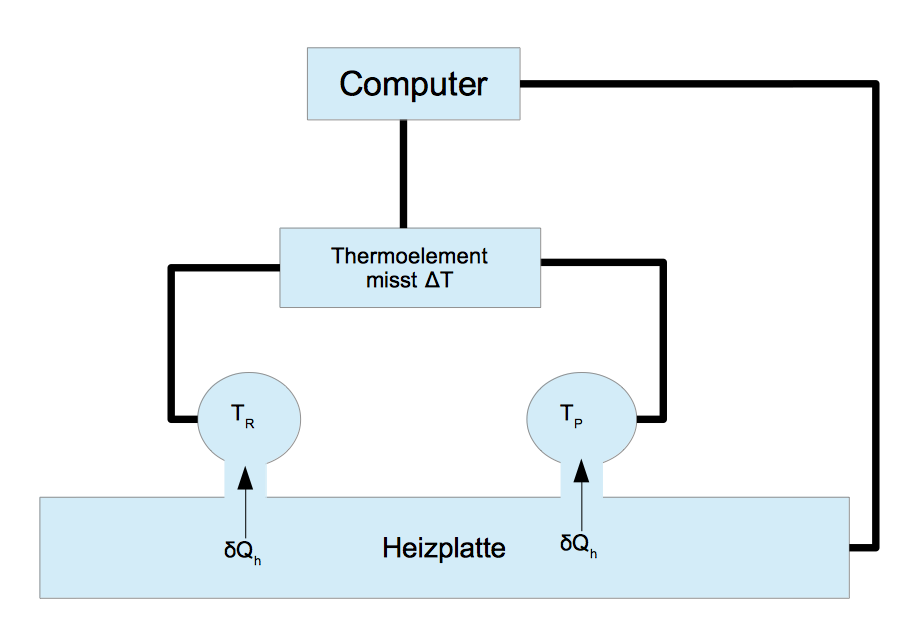
\includegraphics[width=13.5cm]{VB_SN.png}
\caption{Der Versuchsaufbau.}
\end{figure} 
\FloatBarrier

\newpage
\subsection{Durchführung}
Das Dynamische Differenzkaloriemeter (DSC) wurde hochgefahren. Dazu wurde die Apparatur durch den Anschluss „Purge” \;mit einem Stickstoffstrom von ca. 50\;ml/min gespült. Der Druck wurde mittels einer Schwebkugel auf einen Wert von 70 eingestellt. Durch den Stickstoffstrom wurde die Kondensation von Wasser in der Athmosphäre, die die Messung beeinflusst hätte, verhindert. Die Probe des Indiummetalls lag in einer „crimp cell” \;vorbereitet vor. Es wurde zuerst Indium gemessen (Messbereich 100~°C -200~°C). Als Referenz wurde ein leeres Aluminiumpfännchen genutzt. Während des Messdurchgangs des Indiums wurde die Probe des Polymethylmethacrylat (PMMA) vorbereitet. Es wurde 19,7\;mg PMMA in eine „sealed cell” \;eingewogen. Die „sealed cell” \;wurde dann mittels einer hydraulischen Presse die Zelle mit einem Aluminium-Plättchen gasdicht verschlossen. Nach Abschluss der Messung des Indiums wurde die PMMA-Probe gemessen (Messbereich 30~°C -140~°C). Während der Messung der PMMA-Probe wurde die Cyclohexan-Probe vorbereitet. Es wurde ca. 0,03\;ml des Cyclohexans mittels Spritze in eine leere „sealed cell” \;gefüllt. Die Zelle wurde wie die PMMA-Probe mit einem Alumium-Plättchen als Deckel und einer hydraulischen Presse gasdicht verschlossen. Da bei der Messbereich der Cyclohexan-Messung unterhalb der Raumtemperatur liegt, wurde die Apparatur zusätzlich mit flüssigen Stickstoff gespült. Der Messbereich lag bei 30~°C- -110~°C und zurück zu 30~°C. Alle Messungen wurden mit einer Heizrate von Heizrate 10~°C/min durchgeführt.\\

\subsection{Differential Scanning Calometry}
Ein "Differential Scanning Calorimeter" (DSC) misst bei gleichmäßiger Wärmezufuhr zu zwei Stoffen die resultierende Temperaturdifferenz $\Delta T$.
Differential Scanning Kalorimeter lassen sich in 2 verschiedene Arten unterteilen: Power Compensation DSC und Heat-Flux DSC (in diesem Versuch verwendet). Bei Ersterem befinden sich Probe und Referenz in zwei verschiedenen Öfen, die auf die gleiche Temperatur geheizt werden. Die dafür aufgebrachten Heizleistungen werden verglichen und daraus die Enthalpiedifferenz $\Delta H$ bzw. die Änderung der molaren Wärmekapazität $\Delta C_\mathrm{m}$ ermittelt.
Beim Heat-Flux DSC wird beiden Stoffen die gleiche Heizleitung $\Delta Q_\mathrm{h}$ zugeführt und die resultierende Temperaturdifferenz mittels Thermoelement gemessen.
Bei einer geringen Temperaturdifferenz kann $C_\mathrm{m}(T)$ als konstant angesehen werden und aus den Differenzen $\Delta Q$ und $\Delta T$ errechnet werden (Gleichung \ref{cp}).\\

DSC findet vor allem in der Polymerchemie Anwendung. Durch die Bestimmung der Glasumwandlungstemperatur kann der Temperaturereich ermittelt werden, in dem das Material bearbeitet werden muss. Grundsätzlich kann Glas aus sehr verschiedenen Stoffen hergestellt werden, weist jedoch auch verschiedene Stabilitäten auf. Gleiches gilt für Kunststoffe. 
Sind $\Delta S$, $\Delta H$, $T_\mathrm{tr}$ und $c_p$ bekannt, so können Reaktionsgeschwindigkeitsgesetze aufgestellt und die benötigten Energien errechnet werden.\\ 
Ferner können auch Kunststoffarten bestimmt werden.
Stoffe mit geordnetem Kristallgitter neigen eher zu einem Phasenübergang erster Ordnung; der "Peak" der DSC- Kurve ist dann relativ schmal. Bei unreinen Gittern ist der Phasenübergang  kontinuierlicher. So können mittels DSC auch Reinheits- und Kristallisationsgrad ermittelt werden.\\



\section{Auswertung}
Die Auswertung der Messergebnisse erfolgte über das Programm \textit{TA60}. Zur Bestimmung der Umwandlungsenthalpie wurde das Integral über den $"$Peak$"$\, bis zur Basislinie gebildet. Am Wendepunkt der $"$Peak$"$-Linie wurde eine Tangente angelegt; der Schnittpunkt dieser mit der Basislinie ergab die Umwandlungstemperatur.\\ 

\subsection{Rechnung}
 
$\Delta S$ ergibt sich aus Gleichung (\ref{S}). Cyclohexan wurde mit steigender und abfallender Temperatur gemessen. Die tabellierten Werte sind die je die Mittelwerte der zugehörigen Kurve. Zur Berechnung wurden die Beträge der Werte der 2. Messung verwendet. Das Vorzeichen bezieht sich somit auf die 1. Messung.\\

\begin{equation}\label{S}
\left(\frac{\Delta H}{T}\right)_p = \Delta S
\end{equation}

Die Ergebnisse sind in Tabelle (\ref{TabelleMesswerte}) dargestellt.\\

\begin{table} [h!] \label{TabelleMesswerte} %hier aktuelle Tabelle
\caption{Messwerte}
\begin{tabular}{c|c|c|c|c}
 & Stoffmenge $n$  & $T_\mathrm{tr}$  &  $\Delta H $ & $\Delta S$ \\ 
& [mol] & [K] & $[\mathrm{J} \cdot \mathrm{mol}^{-1}]$& [J $\cdot$ K$^{-^1}\cdot$mol$^{-1}$] \\
\hline 
Indium & $232 \cdot 10^1$ & 432 &  322 $\cdot 10^1$ & 7,45 \\ 
\hline 
PMMA 1.Peak & $1152 \cdot 10^2$ & 360,22 -397,43 &  - & - \\
&&Mid Point: 361,68&&\\ 
\hline 
Cyclohexan 1.Übergang & 279 & 278,85 & 1711 & 6,14 \\ 
Cyclohexan 2.Übergang & 279 & 187,4& 4111 & 21,9 \\
\end{tabular}
\end{table}
\FloatBarrier

Indium zeichnet sich in der festen Phase durch eine starke Regelmäßigkeit aus, sodass ein klassischer fest-flüssig Übergang (Phasenübergang 1. Ordnung) stattfand.\\
 
 Bei PMMA sind wie zu erwarten 2 Peaks zu sehen. Da es sich bei PMMA um einen Phasenübergang 2. Ordnung handelt, kann nur der entsprechende Temperaturbereich ermittelt werden, nicht jedoch $\Delta H$ und $\Delta S$. Hier ist ein Glasübergang, d.h. ein Phasenübergang 2. Ordnung aufgetreten. Dabei ist die Änderung der Entropie stetig und es bildet sich kein Phasengleichgewicht mit unterschiedlichen Phasen. Anfangs- und Endpunkte des $"$Übergangs$"$\, sind somit nicht genau definiert.\\
  
Cyclohexan zeigt in der Kurve jeweils 2 $"$Peaks$"$\, und demnach auch 2 Phasenübergänge: flüssig-fest1-fest2 und zurück. Auch hier handelt es sich um Phasenübergänge 1. Ordnung. Die festen Phasen weisen unterschiedliche Kristallstrukturen auf.\\
 
\section{Fehlerdiskussion}

Die Mess- und Literaturwerte sind in Tabelle (\ref{TabelleMesswerte}) und (\ref{TabelleLiteraturwerte}) dargestellt.


\begin{table} [h!] \label{TabelleLiteraturwerte}
\caption{Literaturwerte} %aktuelle Tabelle :)
\begin{tabular}{c|c|c|c|c}
  & $T_\mathrm{tr}$  & $\Delta H$  & $\Delta S$ \\ 
 & [K] & [J$\cdot$mol$^{-1}$] & [J $\cdot$ K$^{-^1}\cdot$mol$^{-1}$] \\
\hline 
Indium & 429,75 \footnotemark &3279 & 7,630 \\ 
\hline 
PMMA & 378\footnotemark& - & -  \\ 
\hline
Cyclohexan 1.Übergang &  279,74 \footnotemark &2676& 9,566\\ 
Cyclohexan 2.Übergang & 186,09 \footnotemark &6741& 36,22\\ 
\end{tabular}
\end{table}
\FloatBarrier

\footnotetext[1]{\emph{CRC Handbook of Chemistry and Physics}, 84. Auflage; D.R. Lide; CRC Press LLC: Boca Raton, \textbf{2004}.}
\footnotetext[2]{\emph{CRC Handbook of Chemistry and Physics}, 84. Auflage; D.R. Lide; CRC Press LLC: Boca Raton, \textbf{2004}.}
\footnotetext[3]{\emph{CRC Handbook of Chemistry and Physics}, 84. Auflage; D.R. Lide; CRC Press LLC: Boca Raton, \textbf{2004}.}
\footnotetext[4]{Kabo, G.J.; Kozyro,A., A.; Frenkel, M.; Blokhin, A. V.\emph{Mol. Cryst. Liq. Cryst.}, \textbf{1999}, \emph{326}, 333-335.}

Für Indium und Cyclohexan liegen die Umwandlungstemperaturen sehr nah an den Literaturwerten (Abweichung $< 0,6\% $); für Cyclohexan ist auch die Abweichung von $\Delta S$ und $\Delta H$ vergleichsweise klein. Für Cyclohexan ergeben sich dagegen Abweichungen von $\Delta H$ und $\Delta S$ von $> 50\%$.\\
Für\,PMMA war nur die "Mid Point$"$-Temperatur des Glasübergangs zu finden. Die Messung zeigt hier eine Abweichung von $4,5\%$.
Da die Messung direkt mit dem Programm erfolgte, kann keine zusätzliche Fehlerrechnung gemacht werden und hier werden ausschließlich systematische Fehler diskutiert.\\

Grobe Fehler können durch zu ungenaues Abwiegen entstanden sein, bzw. dadurch, dass die Kapseln den Rand berührten. In dem Fall kann es sein, dass durch das Gerät mehr Wärme hinzugefügt wird als der Referenz und dabei mit der gleichen zugefügten Wärme gerechnet wird. Dies führt zu einer geringeren Enthalpie, wie auch im Vergleich zu den Literaturwerten sichtbar ist. Dieser Fehler könnte die starke Abweichung der Enthalpie im Vergleich zur relativ genauen Temperatur erklären. Da dieser Unterschied besonders bei Cyclohexan auffällig ist, gibt es hier noch eine andere Erklärungsmöglichkeit:
Cyclohexan ist eine sehr flüchtige Substanz und konnte nach dem Wiegen vielleicht durch undichte Stellen teilweise aus der Kapsel entweichen. Die Substanzmenge wurde nur zur Berechnung der Enthalpien verwendet und spielte bei den Temperaturen keine Rolle (Oder aber beim Abwiegen traten Fehler auf). \\
 Ebenfalls eine mögliche (schwer überprüfbare) Fehlerquelle ist die Genauigkeit der Referenzmasse bzw. -reinheit.\\

Bei PMMA trat dieser Fehler gar nicht erst auf, da es nicht möglich ist, Enthalpie und somit auch Entropie zu bestimmen. Die Enthalpie wurde in den anderen Messungen durch Integration über den "Peak"\, bestimmt, dh. bei definierter Anfangs- und Endtemperatur. Bei PMMA würde dabei jedoch über eine $"$Stufe$"$ integriert werden. Dadurch, dass die Polymere sehr unterschiedliche Längen aufweisen und keine Probe die gleiche Anordnung und Zusammensetzung hat und außerdem der Übergang nach der 2. Ordnung stattfindet, ist die Anfangs- und Endtemperatur schwer bestimmbar und auch nicht allgemein aussagekräftig. Die Messung mit PMMA und anderen Polymeren ist daher nicht sehr genau. \\
Wie auch erwartet, wurden zwei Glasübergangstemperaturen gemessen, jedoch wäre die Auswertung beider wissenschaftlich nicht genau. Zunächst kann es sein, dass die einzelnen Polymere durch ihre sehr unterschiedliche Länge und Lage anders von der zugefügten Wärmemenge erreicht wurden. So fand vielleicht ein Übergang nur für einen Teil statt und anders verzweigte oder auch verunreinigte Bereiche der Probe brauchten mehr Wärme, um auch den Phasenübergang zu erreichen. Dass der Literaturwert dennoch kleiner ist, spielt keine signifikante Rolle, da auch die Molmasse des Polymers lediglich einen Mittelwert darstellt. Außerdem können auch die Literaturwerte nicht als absolut gesehen werden, sondern sind ebenfalls fehlerbehaftet bzw. wurden vielleicht mit anderen Methoden bestimmt.\\ 

Zur Berechnung wird außerdem $C_{\mathrm{m},p}(T)$ als konstant angesehen, da Phasenübergänge 1. Ordnung bei einer definierten Temperatur stattfinden. Der "Peak$"$ in der Auftragung bei Indium müsste deutlich schmaler sein. Dies ist wahrscheinlich durch eine zu hohe Heizrate entstanden. Das Phasengleichgewicht konnte sich demnach nicht einstellen und die Messung ist zu ungenau. Dadurch ist auch die Annahme der konstanten Wärmekapazität nicht korrekt. Da das Programm jedoch das Integral über den Flächeninhalt bildet, muss der Peak eine gewisse Breite haben, damit die Enthalpie auf diese Weise berechnet werden kann. Die Auswirkung dieses Fehlers ist also wahrscheinlich nicht sehr groß.\\

\section{Literaturverzeichnis}
1\quad Eckhold, Götz: \emph{Praktikum I zur Physikalischen Chemie}, Institut für Physikalische Chemie, Uni Göttingen, \textbf{2014}.

\vspace{0,5 cm}

2 \quad Eckhold, Götz: \emph{Statistische Thermodynamik}, Institut für Physikalische Chemie, Uni Göttingen, \textbf{2012}.

\vspace{0,5cm}

3 \quad Eckhold, Götz: \emph{Chemisches Gleichgewicht}, Institut für Physikalische Chemie, Uni Göttingen, \textbf{2015}.\\

\vspace{0,5cm}

4 \quad Atkins, P.W.: \emph{Physikalische Chemie}, Wiley-VCH, Weinheim, \textbf{2006}.\\

\vspace{0,5cm}

5 \quad Zemansky: \emph{Heat and Thermodynamics},Mc Graw-Hill, New York, \textbf{1990}.\\

\end{document}
